%%%%%%%%%%%%%%%%%%%%%%%%%%%%%%%%%%%%%%%%%
% Short Sectioned Assignment
% LaTeX Template
%%%%%%%%%%%%%%%%%%%%%%%%%%%%%%%%%%%%%%%%%

%----------------------------------------------------------------------------------------
%   PACKAGES AND OTHER DOCUMENT CONFIGURATIONS
%----------------------------------------------------------------------------------------

\documentclass[paper=a4, fontsize=11pt]{article} % A4 paper and 11pt font size

\usepackage[T1]{fontenc} % Use 8-bit encoding that has 256 glyphs
\usepackage{fourier} % Use the Adobe Utopia font for the document - comment this line to return to the LaTeX default
\usepackage[english]{babel} % English language/hyphenation
\usepackage{amsmath,amsfonts,amsthm} % Math packages

\usepackage{sectsty} % Allows customizing section commands
\allsectionsfont{\raggedright \normalfont\scshape} % Make all sections centered, the default font and small caps

\usepackage{fancyhdr} % Custom headers and footers
\pagestyle{fancyplain} % Makes all pages in the document conform to the custom headers and footers
\fancyhead{} % No page header - if you want one, create it in the same way as the footers below
\fancyfoot[L]{} % Empty left footer
\fancyfoot[C]{} % Empty center footer
\fancyfoot[R]{\thepage} % Page numbering for right footer
\renewcommand{\headrulewidth}{0pt} % Remove header underlines
\renewcommand{\footrulewidth}{0pt} % Remove footer underlines
\setlength{\headheight}{13.6pt} % Customize the height of the header

\usepackage{parskip}
\setlength{\parindent}{15pt}
\usepackage{graphicx}

\usepackage{booktabs}
\newcommand{\ra}[1]{\renewcommand{\arraystretch}{#1}}

%\numberwithin{equation}{section} % Number equations within sections (i.e. 1.1, 1.2, 2.1, 2.2 instead of 1, 2, 3, 4)
%\numberwithin{figure}{section} % Number figures within sections (i.e. 1.1, 1.2, 2.1, 2.2 instead of 1, 2, 3, 4)
%\numberwithin{table}{section} % Number tables within sections (i.e. 1.1, 1.2, 2.1, 2.2 instead of 1, 2, 3, 4)

\setlength\parindent{0pt} % Removes all indentation from paragraphs - comment this line for an assignment with lots of text

%----------------------------------------------------------------------------------------
%   TITLE SECTION
%----------------------------------------------------------------------------------------

\newcommand{\horrule}[1]{\rule{\linewidth}{#1}} % Create horizontal rule command with 1 argument of height

\title{ 
\normalfont \normalsize 
\textsc{Nuclear Engineering, UC Berkeley} \\ [25pt] % Your university, school and/or department name(s)
\horrule{0.5pt} \\[0.4cm] % Thin top horizontal rule
\huge HW4 for Numerical Simulation of Radiation Transport\\ % The assignment title
\horrule{2pt} \\[0.5cm] % Thick bottom horizontal rule
}

\author{Xin Wang} % Your name

\date{\normalsize\today} % Today's date or a custom date

\begin{document}

\maketitle % Print the title




\section*{Problem 1}
Calculate an integration $I = \int_{x_{min}}^{x_{max}}f(x) dx$ using rejection Monte Carlo method procedures:

1) Sample random points in the rectangle area [xmin, xmax]*[0, fmax]:

\begin{eqnarray}
x_p = x_{min} + (x_{max}-x_{min})*\xi_1 \nonumber\\
y_p = 0 + fmax * \xi_2
\end{eqnarray}

2) For each random point P (px, py), check if it's under the function curve, i.e. if $y_p \leq f(x_p)$.
If this is true, accept the point, otherwise reject the point. 

3) The probability for a point to be accepted is approximately 
\begin{eqnarray}
prob = \frac{N_{accept}}{N_{tot}}
\end{eqnarray}

4) The integral is I = Area * prob where Area = (xmax- xmin)*fmax

Assuming the true value for $\pi$ is 3.14159, the result for $\pi = 4\int_0^1 sqrt(1-x^2) dx$ and $\pi = 4\int_0^1 \frac{1}{1+x^2}$ with different numbers of samples is listed in table \ref{pb1}:

\begin{table*}[h]\centering
\ra{1.3}
\begin{tabular}{@{}cccc@{}}\toprule
  & nb & f1 relative error & f2 relative error \\ \midrule
    & 10         & 0.036     &0.108 \\
    & 100        & 0.082    &0.0196 \\
    & 1000         & 0.0186 & 0.0377 \\
    & 10000        & 0.0025 & 0.0013 \\
\bottomrule
\end{tabular}
\caption{Relative error of rejection Monte Carlo method for integral calculation}
\label{pb1}
\end{table*}

\clearpage

\section*{Problem 3}
b) 
The flux distribution in the slab for different number of source photons are plotted in figure \ref{flux_plot}. The flux distribution in the slab from SN code and Monte Carlo code are plotted in figure \ref{flux_plot_sn}.

\begin{figure}
    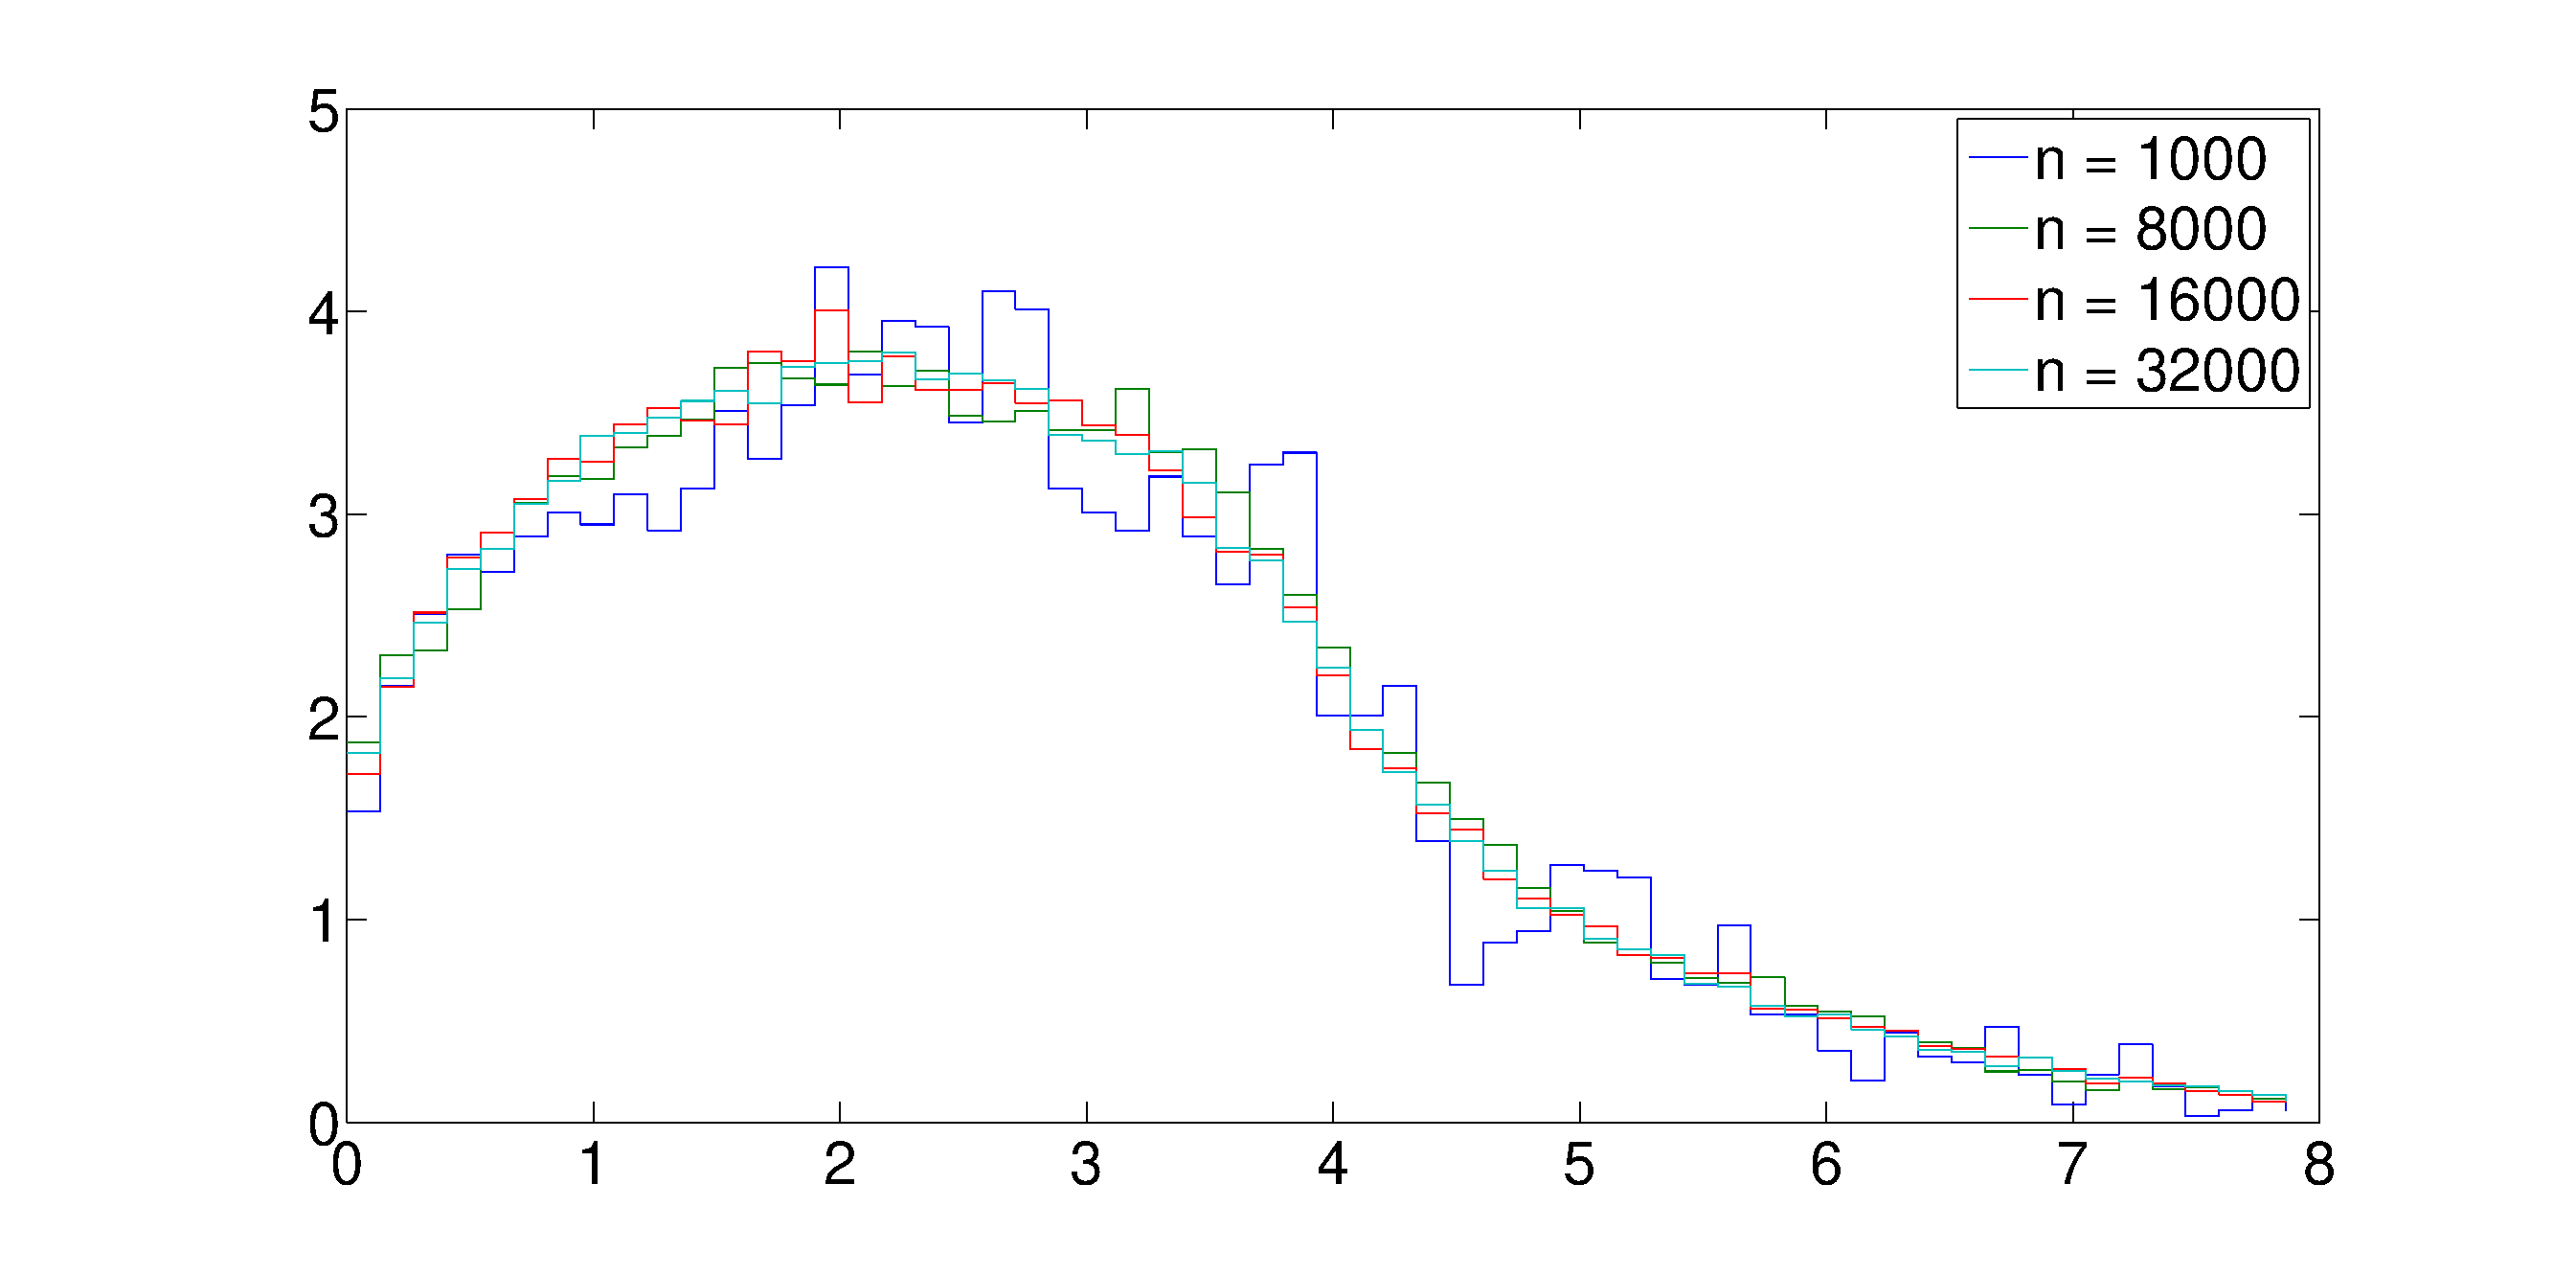
\includegraphics[width = \textwidth]{flux_plot.eps}
    \caption{Pb3: Flux distribution in the slab}
    \label{flux_plot}
\end{figure}

\begin{figure}
    \includegraphics[width = \textwidth]{flux_plot_sn.eps}
    \caption{Pb3: Comparison of flux distribution in the slab with SN code}
    \label{flux_plot_sn}
\end{figure}

c) The outgoing partical current at the left courdary is 0.8085, and at the right boundary is 0.0569. The results from SN code was 0.8234 and 0.0582. 
The absorption rate in the left half of the slab is 2.57, in the right half is 0.56. The absorption rates are 2,54 and 0.56 in SN code.

d) and e) The escape probabilities through the left and right boundaries and the absorption probabilities in the left and right half of the slab from the Monte Carlo code and SN code are compared in table \ref{pb3}. The result from Monte Carlo method and from SN method agree with each other. 

\begin{table*}[h!]\centering
\ra{1.3}
\begin{tabular}{ccccc}\toprule
 $N_{TOT}$ & $P_{escR}$ & $P_{escL}$ & $P_{absR}$ &$P_{absL}$ \\ \midrule
  125   & 0.0080 & 0.2160 & 0.6080 & 0.1680 \\
  250   & 0.0200 & 0.1600 & 0.6520 & 0.1680\\
  500   & 0.0120 & 0.1820 & 0.6840 & 0.1220\\
  1000  & 0.0120 & 0.2070 & 0.6430 & 0.1470\\
  2000  & 0.0135 & 0.1985 & 0.6450 & 0.1430\\
  4000  & 0.0173 & 0.2070 & 0.6318 & 0.1440\\
  8000  & 0.0174 & 0.2086 & 0.6310 & 0.1417\\
  16000 & 0.0158 & 0.2048 & 0.6378 & 0.1393\\
  32000 & 0.0137 & 0.2064 & 0.6407 & 0.1432\\
  64000 & 0.0147 & 0.2064 & 0.6358 & 0.1430\\
  SN    & 0.01455 & 0.2058 & 0.6367 & 0.1420\\
\bottomrule
\end{tabular}
\caption{Pb3: Comparison of escape probabilities and absorption probabilities in the slab}
\label{pb3}
\end{table*}

\clearpage
\section*{Problem 4}
The procedures to calculate the energy reflection factor(albedo) for a beam of 2Mev photons normally incident on a face of a slab of ordinary concrete, 5cm thick is the following:

a) The photon from the beam incident to the face of the slab, at z0=0 with the angle $\mu = 1$. 

The total collision cross section can be found online as attenuation coefficient:
\begin{eqnarray}
\rho_{concrete} = 2.3 (g/cm^3) \nonumber\\
\Sigma_{tot} = 4.557 * 0.01 * \rho (cm ^{-1})
\end{eqnarray}

Sample the distance to collision:
\begin{equation}
dist = -\mu/\Sigma_{tot} ln(\xi_3)
\end{equation}

b) So the first interaction would be at $z1 = z0 + dist = dist$ if z1 is within the slab [0, 5]cm. If Z1 is not within [0, 5]cm, then score zero

c) If Z1 is within [0, 5]cm, determine the collision type (absorption or scattering):
To do so, we need to at first calculate the scattering cross section. The microscopic total Compton scattering cross section can be obtain as:
\begin{eqnarray}
\sigma _{cs} &=& 2 \pi r_0 \{ \frac{1+\alpha} {\alpha ^2} [\frac{2(1+\alpha)}{1+2\alpha} - \frac{1}{\alpha} ln(1+2\alpha)] + [\frac{1}{2\alpha} ln(1+2\alpha) - \frac{1+3\alpha}{(1+2\alpha)^2}] \} [cm^2] \nonumber\\
\alpha &=& \frac{E_{in}}{m_0 c^2} \nonumber\\
r_0 &=& \frac{e^4}{(m_0 c^2)^2}
\end{eqnarray}

The macroscopic Compton scattering cross section is:
\begin{eqnarray}
\Sigma_{cs} = \sigma{cs} * N
\end{eqnarray}

The atomic number density N can be calculated from :

\begin{eqnarray}
N = \rho * Av/ A
\end{eqnarray}

The average atomic mass A for ordinary concrete can be calculated from the material composition in table \ref{concrete_material_composition} and the Z/A ratio for ordinary concrete is 0.50932. 

\begin{table*}\centering
\ra{1.3}
\begin{tabular}{@{}ccc@{}}\toprule
    & isotope Z & weight fraction(\%) \\ \midrule
    & 1         & 0.022100 \\
    & 6         & 0.002484 \\
    & 8         & 0.574930 \\
    & 11        & 0.015208 \\
    & 12        & 0.001266 \\
    & 13        & 0.019953 \\
    & 14        & 0.304627 \\
    & 19        & 0.010045 \\
\bottomrule
\end{tabular}
\caption{Ordinary concrete composition}
\label{concrete_material_composition}
\end{table*}


d) If absorbed, i.e. $\xi > Pcs = \frac{sigma_cs}{sigma_tot}$, score zero. Otherwise the photon is scattered. Sample the scattered photon energy E1 as shown in the flow chart and calculate the scattered angle $cos\theta _1$.

\begin{eqnarray}
cos(\theta_s) = 1 - \lambda_1 + \lambda_0\\
m_0 c^2 = 0.511 Mev\\
\lambda_0 = \frac{m_0 c^2}{E_0}
cos(\theta_1) = cos(\theta_0) cos(\theta _ s) + sin(\theta_0) sin(\theta _ s) cos(\beta)
\end{eqnarray}

e) If scattering anble is smaller or equal to 90, then the photon will not go back without another scattering. It doens't contribute significantly to the reflection process.

f) If the scattering angle is larger than 90, calculate the second interaction distance s2.

g) If $s2 < \|x_1/cos(\theta_1)\|$, the photon has the second interaction in the slab. It doesn't contribute significantly to the reflection process.

h) If $s2 geq\|x_1/cos(\theta_1)\|$, the photon reflects back with a single scattering. Score $E_1/ cos(\theta_1)$

The energy reflection factor (albedo) is $Score/ N_{source} = 0.17\% $. 
\end{document}